\section{Static and Dynamic Requests}
% \meta{Describe how static and dynamic files are served}
Serving static and dynamic content was developed as two seperate features and
handler classes \texttt{StaticHandler} and \texttt{DynamicHandler}, but
later merged into what is now the \texttt{RequestHandler} class. From the
beginning it was clear that the handler classes would have much functionality
such as reading the request, invoking the parser and returning the response in
common, but also some distinct functionality. A good way to vary an algorithm
whilst keeping much of the functionality the same is to use the Template
Method design pattern. The process of handling requests can be split up into
the following steps:

\begin{enumerate}
  \item Parse the request
  \item Prepare the response
  \item Return the reponse to the client
  \item Close the connection
\end{enumerate}

Given this process, the part that differs between handling static and dynamic
files is preparing the response. The Template Method makes provides a
convenient way to vary the implementation of how the response is prepared
\cite{design_patterns}.
Figure~\ref{template} shows how the relationship between the handler classes.

\begin{figure}[htb]
  \centering
  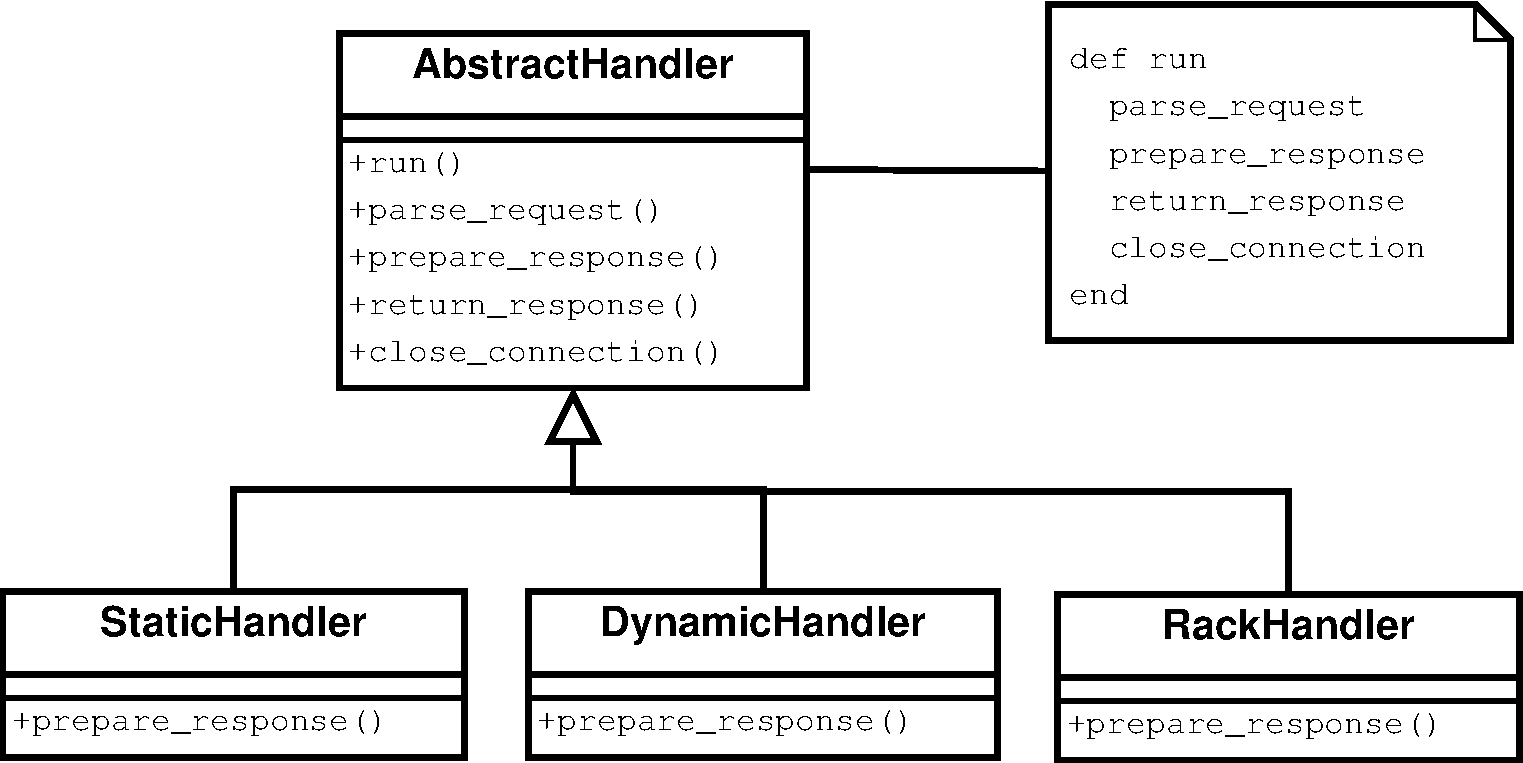
\includegraphics[width=0.7\textwidth]{diagrams/handlers.pdf}
  \caption{Initial handler implementation using the Template Method.}
  \label{template}
\end{figure}

Invoking run on each handler class would then follow the same process, but
each have their own implementation of \texttt{prepare\_response} method. Once
both handler classes were implemented it became clear that it would make more
sense to merge the two together to mirror how Yarn can be run to serve either
static and dynamic files or a Rack application. Figure~\ref{template2} shows
how the final handler classes were implemented (\texttt{RackHandler} is
covered in Section~\ref{rack}).

\begin{figure}[htb]
  \centering
  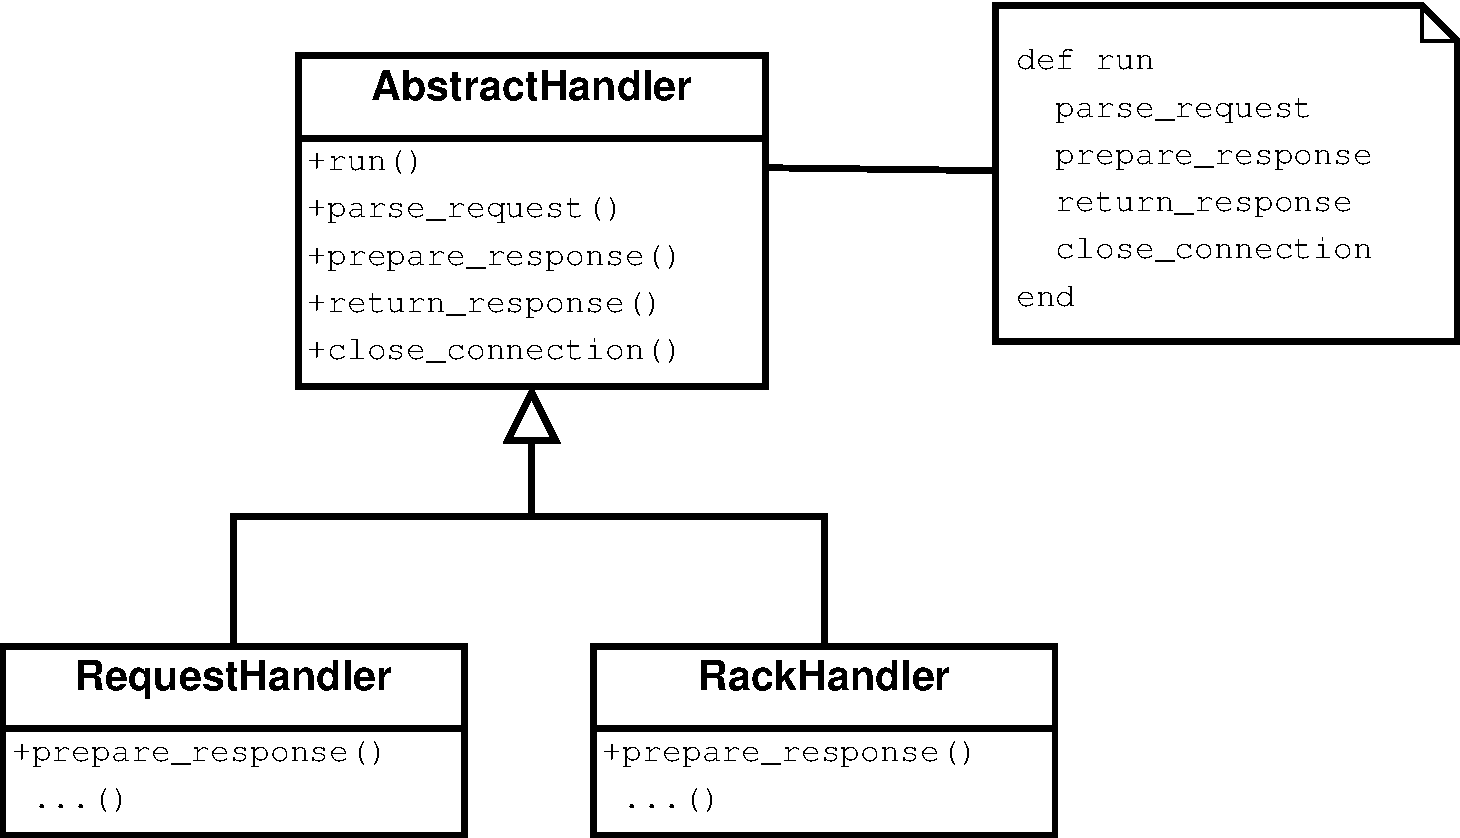
\includegraphics[width=0.7\textwidth]{diagrams/handlers2.pdf}
  \caption{Final handler implementation using the Template Method.}
  \label{template2}
\end{figure}

\subsection{RequestHandler}
\label{reqhandler}
The \texttt{RequestHandler} works by checking whether the requested path is a
file or a directory. Listing~\ref{reqhandle} show the logic
determining what is being served.

\begin{lstlisting}[label=reqhandle,caption=\texttt{RequestHandler} logic.
(lib/yarn/request\_handler.rb:8)]
begin
  if File.directory?(path)
    serve_directory(path)
  elsif File.exists?(path)
    path =~ /.*\.rb$/ ? serve_ruby_file(path) : serve_file(path)
  else
    serve_404_page
  end
rescue ProcessingError
  log "An error occured processing #{path}"
  serve_500_page
end
\end{lstlisting}

If the requested path is a directory, then a directory listing is served. In
case the requested file is ends with \texttt{.rb}, then it is executed and the
result is returned. In case the file does not exist or an error occurs
executing a Ruby file, then an error page is returned. Ruby files are executed
in the \texttt{execute\_script} method by evaluating the file using a new Ruby
VM and the result stored as the response body.


